\documentclass{beamer}

% Top-aligning columns within a top-aligned frame
% https://tex.stackexchange.com/questions/16447/beamer-top-aligning-columns-within-a-top-aligned-frame
\makeatletter
\newenvironment{myitemize}{%
   \setlength{\topsep}{0pt}
   \setlength{\partopsep}{0pt}
   \renewcommand*{\@listi}{\leftmargin\leftmargini \parsep\z@ \topsep\z@ \itemsep\z@}
   \let\@listI\@listi
   \itemize
}{\enditemize}
\makeatother  

\usepackage[USenglish]{babel}
\usepackage[utf8]{inputenc}
\usepackage{amssymb, amsmath}
\usepackage{bm}
\usepackage{color}
\usepackage{tikz}
\usepackage{url}

\definecolor{links}{HTML}{2A1B81}
\hypersetup{colorlinks,linkcolor=,urlcolor=links}

\usetheme{Boadilla}

\bibliographystyle{apalike}
% make bibliography entries smaller
%\renewcommand\bibfont{\scriptsize}
% Now get rid of all the colours
\setbeamercolor*{bibliography entry title}{fg=black}
\setbeamercolor*{bibliography entry author}{fg=black}
\setbeamercolor*{bibliography entry location}{fg=black}
\setbeamercolor*{bibliography entry note}{fg=black}

\newcommand{\lnorm}[1]{\left\lVert#1\right\rVert^2}
\newcommand{\norm}[1]{\left\lVert#1\right\rVert}

% and kill the abominable icon
\setbeamertemplate{bibliography item}{}

\begin{document}
\title[MLP-Mixer]{MLP-Mixer: An all-MLP Architecture for Vision
Ilya}  
\author{Radek Bartyzal}
\date{15. 6. 2021} 
\institute{GLAMI AI}

\frame{\titlepage} 

%--------- END Frame 12 -------------
\begin{frame}{Motivation}

Paper is by Google Brain from 2021.
\vfill

\textbf{Goal}:
Learn useful representations of images.
\vfill
\textbf{Contribution}:
Competitive model using only MLPs = fully connected FF layers with non-linearities.


\end{frame}
%--------- END Frame 12 -------------
\begin{frame}{MLP-Mixer}

\begin{figure}[h]
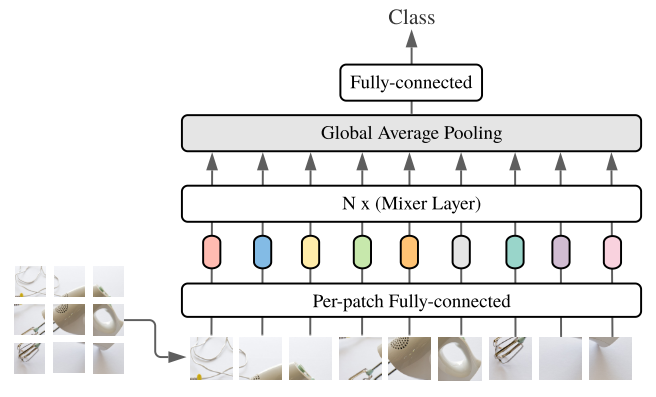
\includegraphics[width=\textwidth]{img/arch}
\end{figure}

\end{frame}

%--------- END Frame 12 -------------
\begin{frame}{MLP-Mixer overall architecture}

\begin{itemize}
\item split image to patches 16x16 pixels
\item pass each patch through \textbf{shared} FC layer to get embedding
\item apply N mixer layers to embeddings
\end{itemize}
\vfill

\begin{itemize}
\item very similar to Visual Transformers
\item mixer block instead of attention between patches
\item per patch FC = Conv layer with stride 16x16 
\end{itemize}
\end{frame}
%--------- END Frame 12 -------------
\begin{frame}{Mixer Block}

\begin{figure}[h]
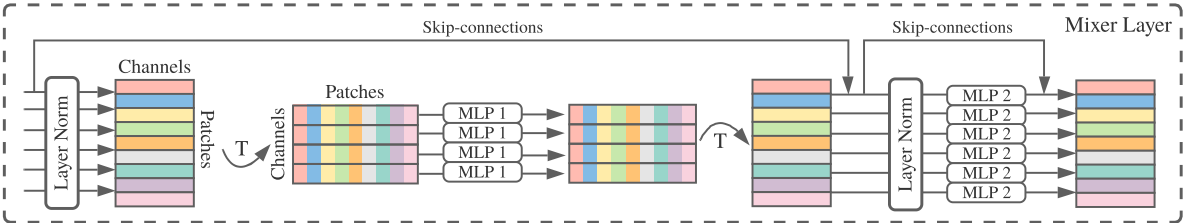
\includegraphics[width=\textwidth]{img/mixer}
\end{figure}

\end{frame}
%--------- END Frame 12 -------------
\begin{frame}{Mixer Block: Token Mixing MLP}

\begin{figure}[h]
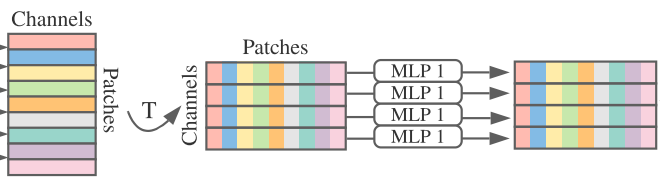
\includegraphics[width=\textwidth]{img/mlp1}
\end{figure}

\begin{itemize}
\item combine information across patches = channel $i$ from all patches
\item same = shared MLP for each channel
\item each channel is some feature detector - because of shared projection of each patch into channels
\end{itemize}

\end{frame}
%--------- END Frame 12 -------------
\begin{frame}{Mixer Block: Channel Mixing MLP}

\begin{figure}[h]
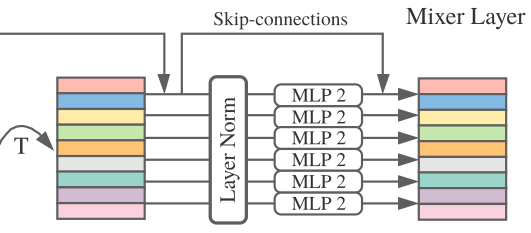
\includegraphics[width=\textwidth]{img/mlp2}
\end{figure}

\begin{itemize}
\item combine information across channels = for each patch separately
\item same = shared MLP for each patch = \textbf{1x1 Conv}
\end{itemize}

\end{frame}
%--------- END Frame 12 -------------
\begin{frame}{MLP Block}

\begin{figure}[h]
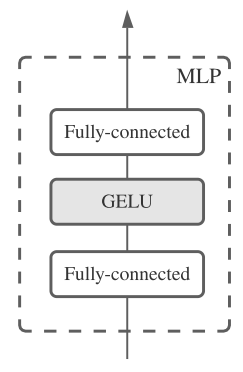
\includegraphics[width=0.3\textwidth]{img/mlp}
\end{figure}

\end{frame}
%--------- END Frame 12 -------------
\begin{frame}{Mixer Block}

\begin{itemize}
\item LayerNorm and skip connections before each \textbf{per patch} operation

\vfill

\item mix information between patches = instead of attention
\item mix information between channels = identical to 1x1 Conv
\item self-attention in ViT does both
\end{itemize}


\end{frame}
%--------- END Frame 12 -------------
%--------- END Frame 12 -------------
\begin{frame}{Models}

\begin{figure}[h]
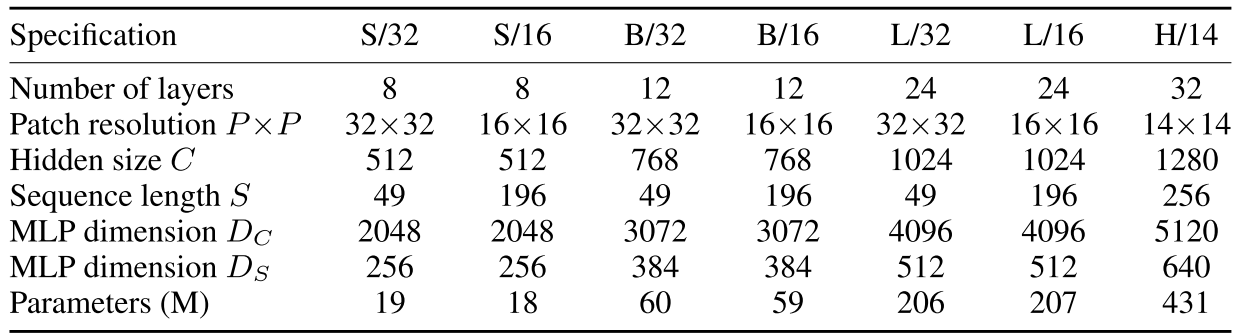
\includegraphics[width=\textwidth]{img/models}
\end{figure}

\end{frame}
%--------- END Frame 12 -------------
\begin{frame}{Fast inference + competitive accuracy}

\begin{figure}[h]
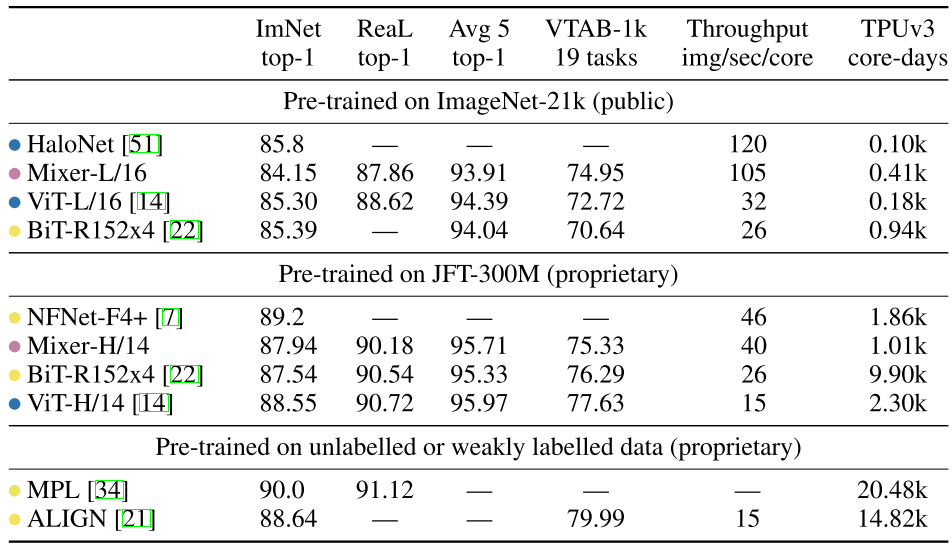
\includegraphics[width=\textwidth]{img/stats}
\end{figure}

\end{frame}
%--------- END Frame 12 -------------
\begin{frame}{Scales very well with more pretraining data}

\begin{figure}[h]
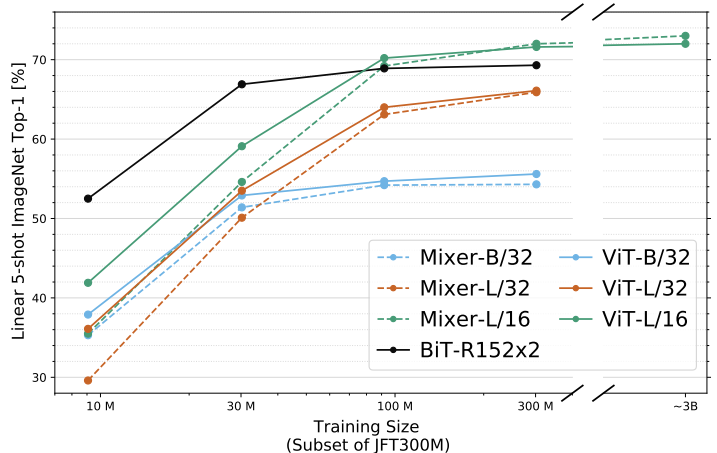
\includegraphics[width=\textwidth]{img/scaling}
\end{figure}

\end{frame}
%--------- END Frame 12 -------------
\begin{frame}{Token Mixing weights in first, second, third layer}

\begin{figure}[h]
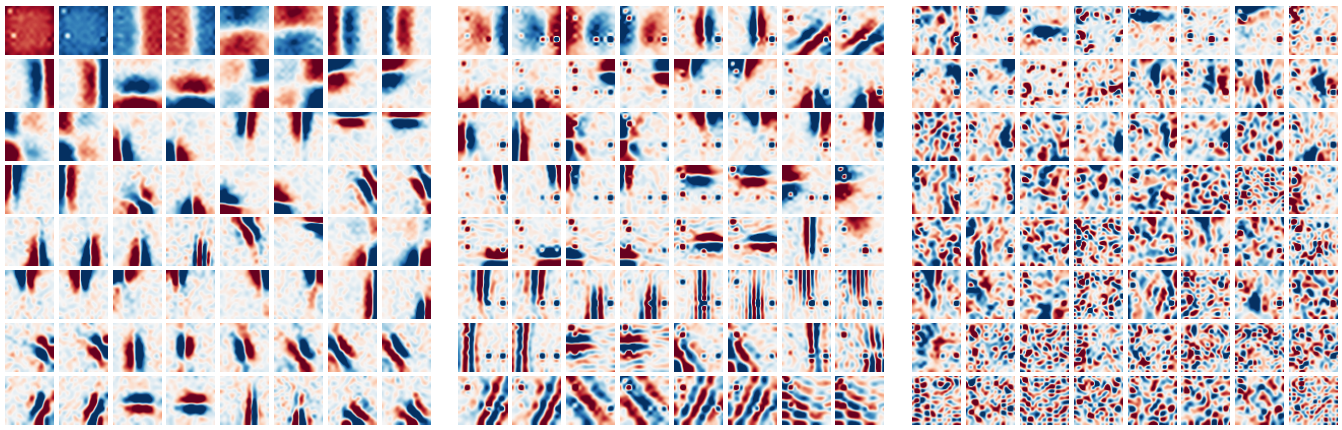
\includegraphics[width=\textwidth]{img/filters}
\end{figure}

\begin{itemize}
\item first layer = edge detector
\item later layers = more complex detectors = like CNN
\end{itemize}

\end{frame}
%--------- END Frame 12 -------------
\begin{frame}{Embedding projection of the patches = patch channels}

\begin{figure}[h]
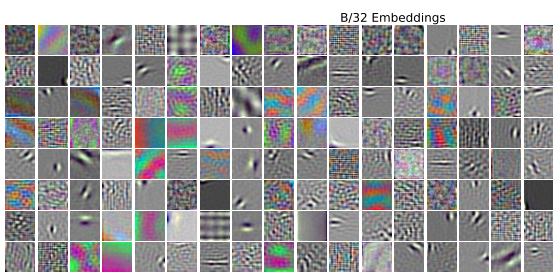
\includegraphics[width=\textwidth]{img/projections}
\end{figure}

\begin{itemize}
\item 32x32 learns nice high level patterns
\item 16x16 (not shown) learns low level noisy patterns
\end{itemize}

\end{frame}
%--------- END Frame 12 -------------
%--------- END Frame 12 -------------
\begin{frame}{Conclusion}


\begin{itemize}
\item uses patches = specific to images, learned projections like CNN
\item separate token and channels mixing
\item fast inference = faster than big ResNet which has better performance
\item competitive accuracy = not a SoTA
\item linear scaling with image size = like CNNs
\item \textbf{best scaling with pretraining dataset size} = biggest advantage
\end{itemize}

\vfill

My 2 cents:
\begin{itemize}
\item adds biases toward images = not a general arch.
\item interesting for efficiency reasons but does not feel like a direction toward a breakthrough
\end{itemize}

\end{frame}
%--------- END Frame 12 -------------
\begin{frame}{Sources}
\begin{thebibliography}{0}

  \bibitem[1]{cit:paper} 1.Tolstikhin, Ilya, et al. "Mlp-mixer: An all-mlp architecture for vision." arXiv preprint arXiv:2105.01601 (2021). \url{https://arxiv.org/abs/2105.01601} 
  
\end{thebibliography}

\end{frame}

 
\end{document}
